\subsection{Energieversorgung} 
Die Elektronik des Dojos bezieht die Energie von einem Akkumulator. Verwendet wird ein Lithiumakkumulator der Marke Trustfire mit einer Nennspannung von $3.7V$. Der Akkumulator besitzt eine Ladungskapazität von $600mAh$.

\subsubsection*{Entladevorgang} 
Der Akkumulator besitzt eine Nennspannung von $4.2V$ bei voller Kapazität und $0V$ \ref{test_Spannungsversorgung} wenn die Kapazität erschöpft ist. Die $0V$ kommen daher zustande, dass der Tiefenentladungsschutz der Batterie die Spannungsversorgung ab einer Spannung unter $2.75V$ kappt. Aus der Batteriespannung wird mit einem Linearregler des Types TL1963A eine $3.3V$ Spannungsversorgung erstellt. Mit dieser Versorgung wird die gesammte Elektronik gespiesen.

\subsubsection*{Ladevorgang}
Der Akkumulator wird über die Spannungsversorgung des USB-Ports geladen. Ein Akkumulator-Management-Chip sorgt dabei für eine konstante Spannung von $4.2V$. Diese Spannung wird benötigt um den Akkumulator zu laden. Die Ladezeit beträgt $2.5h$, siehe Messungen Ladevorgang \ref{sec:Ladevorgang}. Somit ist es möglich, den Akkumulator über eine Nacht komplett zu laden, oder ihn zwischen den Benützungen einmal zu laden. 

\subsubsection{Messungen}
Um die Energieversorgung zu verifizieren wurden 3 verschiedene Messungen durchgeführt. Es wurde der Lade- und Entladevorgang aufgezeichnet, sowie die maximale mögliche Last ausgemessen.

\subsubsection*{Maximale Last}
Um herauszufinden welche Leistung bereitgestellt werden kann, wurde die Energieversorgung mit verschiedenen Lasten betrieben. 

\begin{table}[h]
\centering
\label{messungen_Energie}
\begin{tabular}{|l|c|c|c|}
\hline
Last [$\Omega$]     & 100   & 50    & 10    \\ \hline
Batteriestrom [$mA$]    & 32.55 & 63.79 & 293.3 \\ \hline
Batteriespannung [$V$] & 3.823 & 3.735 & 2.979 \\ \hline
Laststrom [$mA$] & 31.06 & 62.03 & 278.1 \\ \hline
Lastspannung [$V$]  & 3.293 & 3.292 & 2.95  \\ \hline
Leistung [$W$]  & 0.124 & 0.238 & 0.874  \\ \hline
\end{tabular}
\end{table}

Diese Daten zeigen, dass mit einer Leistung von $1W$ die Versorgungsspannung des Printes lediglich auf $2.95V$ sinkt. Dies entspricht einem Spannungsverlust von  $0.35V$, was in der Tolleranz aller elektronischen Bauteile liegt. Da auf unserem Print die maximale Last nur zwischen $0.3 - 0.5W$ liegt, treten keinerlei Probleme auf.
\newpage


\subsubsection*{Entladevorgang}
Um die Batterie zu entladen wurde eine $30\Omega$ Last angeschlossen und dabei ein Entladestrom von $100mA$ erreicht. Dieser Entladestrom entspricht der Leistung, die verbraucht wird, wenn der Print ein Audiofile abspielt. Die Messungen wurde bis zur vollständigen Entladung vollzogen. 
In den Abbildungen \ref{fig:SpannungZuZeit} und  \ref{fig:SpannungZuLadung} ist die Entladekurve für die Spannung im Vergleich zur Zeit und zur Ladung abgebildet:

\begin{figure}[h]
	\centering
	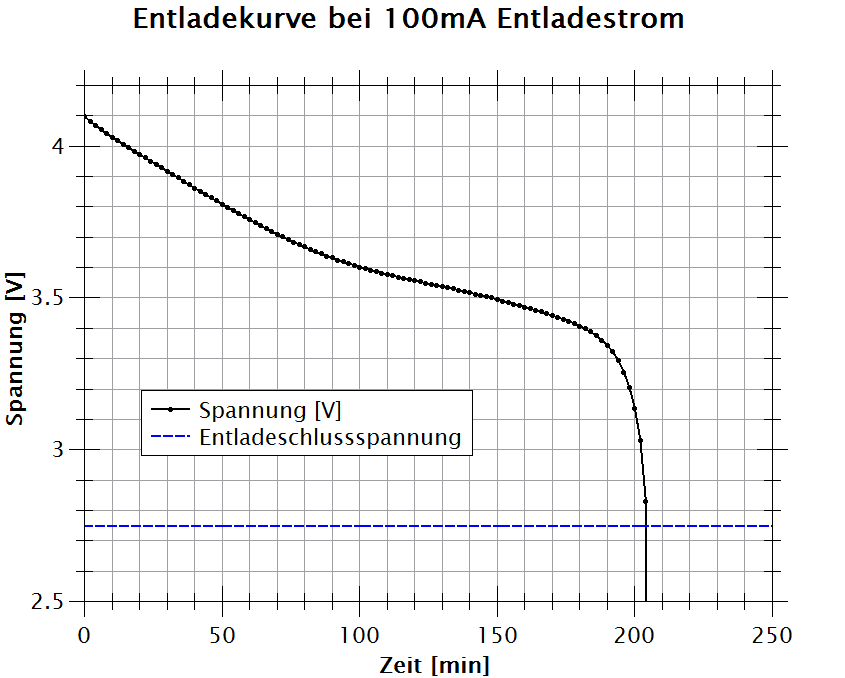
\includegraphics[width=\textwidth]{graphics/SpannungzuZeit.png}
	\caption{Entladekurve bei einer Belastung von 30$\Omega$}
	\label{fig:SpannungZuZeit}
\end{figure}

Wie in der Abbildung \ref{fig:SpannungZuZeit} ersichtlich, hat die Batterie ein Tiefenentladungsschutz bei $2.75V$. Sobald diese Spannung erreicht ist, wird die Spannungsversorgung gekappt, und die Spannung sinkt auf $0V$.\\
Die gesammte Entladung dauert $3h 26min$. Dies entspricht der Laufzeit, die erreicht wird, wenn der Dojo permanent Audiofiles abspielt.

\newpage

\begin{figure}[h]
	\centering
	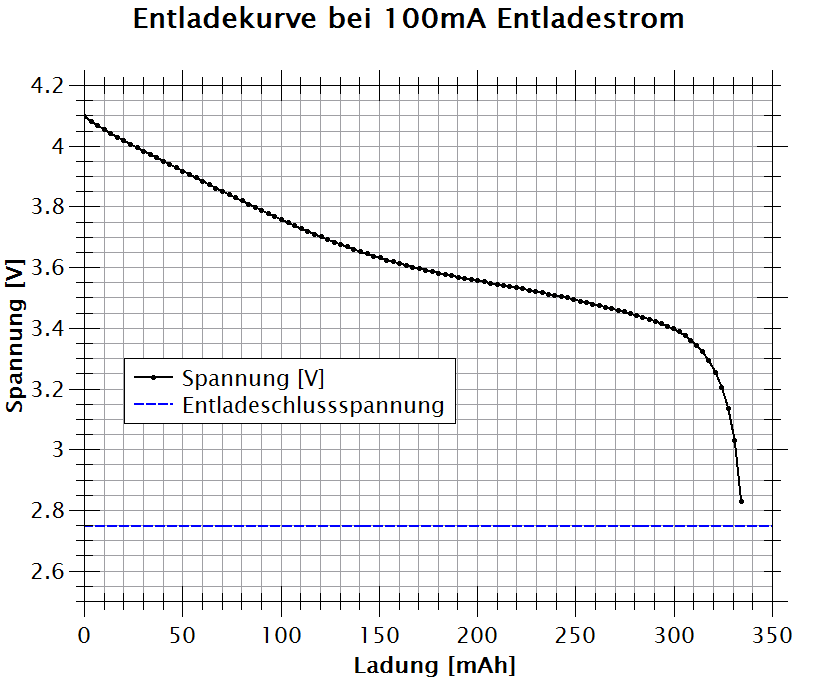
\includegraphics[width=\textwidth]{graphics/SpannungzuLadung.png}
	\caption{Spannung im Verhältnis zur Ladung. Bei einem Widerstand von 30$\Omega$}
	\label{fig:SpannungZuLadung}
\end{figure}

Die Abbildung \ref{fig:SpannungZuLadung} zeigt die abgegebene Ladung im Vergleich zur Batteriespannung. Sie zeigt, dass bei einem Belastung von 100mA die Ladung der Batterie $334mAh$ beträgt. Dies entspricht nicht der angegebenen Ladungskapazität von 600mAh, die der Hersteller verspricht. Die Messung zeigt uns, das der Hersteller die Angaben zu optimistisch ermittelt hat.

\newpage

\subsubsection*{Ladevorgang}
\label{sec:Ladevorgang}
Beim Aufladen der Batterie wurde eine Spannung von $5V$ verwendet. Dabei wurde vor dem Anschliessen der Batterie ein Strom von $1.25mA$ gemessen. Die Ladekurve ist in der Abbildung                       \ref{fig:Ladeleistung} ersichtlich.

\begin{figure}[h]
	\centering
	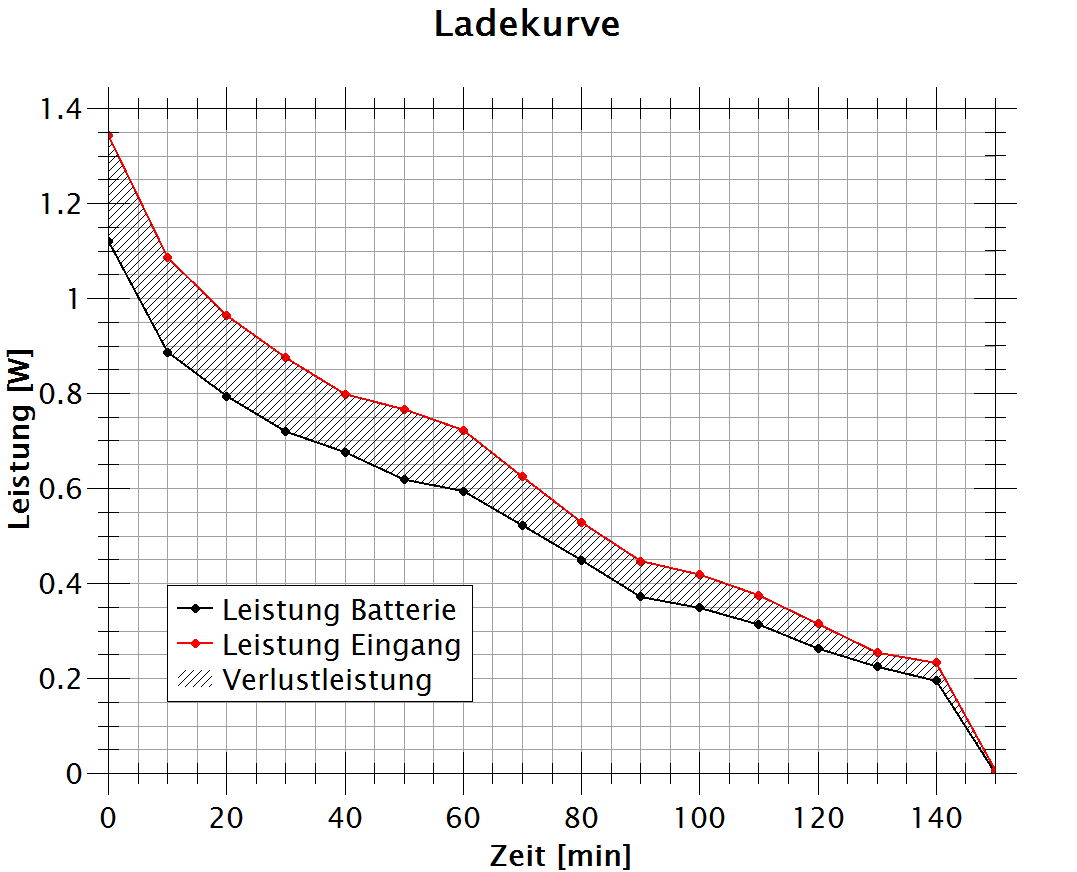
\includegraphics[width=\textwidth]{graphics/ladekurve.png}
	\caption{Ladekurve bei einer konstanten Eingangspannung von 5V}
	\label{fig:Ladeleistung}
\end{figure}

Die gestrichelte Fläche repräsentiert die Verlustleistung beim Laden des Dojos.
Wir erhalten einen Wirkunsggrad von
\begin{equation}
\eta = 83.39%
\end{equation}
Das komplette Aufladen der Batterie dauerte $2.5h$. Somit kann das Museum den Dojo über Nacht problemlos aufladen. Auch Aufladungen zwischen Besuchen können so realisiert werden.